\chapter{Evaluation\label{chapter:evaluation}}

This chapter evaluates the inductive behavior model synthesis technique presented in the previous chapter. Section~\ref{chapter:evaluation-object} makes the evaluation \emph{object} and \emph{objectives} fully precise, by answering \emph{what} is to be evaluated exactly and \emph{why} it is evaluated. The evaluation approach is then presented in Section~\ref{section:evaluation-approach}. Evaluation experiments are described in Section~\ref{section:evaluation-experiments} and results discussed in Section~\ref{section:evaluation-discussion}, which closes this chapter and paves the way to the next one.

Note: This chapter revisits evaluations previously published in~\cite{Damas:2006}, \cite{Dupont:2008} and \cite{Lambeau:2008}. The reader familiar with that material will find here a unified overview of those evaluations, including important ``bug fixes'' as well as clarifications.

\section{Object and Objectives\label{chapter:evaluation-object}}

Let us discussing the objectives of this evaluation first. Our main aim is to answer --~or at least, to set the basis for answering~-- qualitative questions about the inductive behavior model synthesis technique presented in the previous chapter: \emph{how well does it work in practice?}, \emph{is it easy to use?}, or \emph{fast enough for practical cases?} or even \emph{would it be a good choice in this particular situation, or for solving this particular problem?}

Stated as such, however, those questions are difficult to answer in absolute terms. The main reason is that there is no such one \emph{inductive behavior model synthesis technique} but, as discussed in Section~\ref{section:inductive-discussion}, rather a general inductive approach on top of which a set of specific features can be additionally plugged: a scoring heuristic for choosing state pairs to merge, an oracle answering membership queries, the injection of domain knowledge and/or control information, and so on. Also, each of these features has a specific impact on the induction approach in terms of accuracy, usability, time, cost, etc. The questions aforementioned actually hide non-functional requirements of this kind, whose need of fulfillment varies from project to project. Therefore, considering inductive synthesis as a whole for answering these questions would certainly fail. In other words, even if one algorithm -- say \emph{X}SM -- existed that would bundle these features altogether, it would not necessarily fit one's need.

For this reason, we take a different approach to the one of evaluating specifical algorithms like QSM or MSM and consider a finer-grained analysis: considering induction features in isolation, we set our evaluation goal to the discovery -- more precisely an assessment illustrated by experiments -- of positive or negative contribution links between induction features and non-functional requirements. Table ~\ref{table:evaluation-contribution-links} -- already populated with known and/or expected contribution links -- illustrates this kind of correlation between our four induction features (from Section~\ref{section:inductive-discussion}) and the following non-functional requirements (following the taxonomy of \cite{VanLamsweerde:2009}):

\begin{description}

\item[Accuracy] How well does the feature help reaching ``good'' behavior models~--~in the \emph{expert judgment} meaning introduced earlier. As one generally would like reaching \emph{high} accuracy, a positive contribution link captures the fact that, given the same initial set of scenarios, behavior models will be more accurate with the feature plugged than without it. 

\item[Usability] Does the feature make the induction approach easier (positive contribution link) or harder (negative contribution link) to use?

\item[Cost] Cost here captures the effort required to fulfill the expectations of the induction technique, in terms of user involvement, availability and/or difficulty of providing specific knowledge, and so on. As \emph{low} cost being often desirable, a positive (resp. negative) contribution link captures the fact that the feature diminishes (resp. increases) the cost of the technique.

\item[Time] As usual -- while not necessarily desirable -- in many software projects, \emph{the faster the better}. A positive (resp. negative) contribution, therefore, indicates that an induction feature helps achieving a faster (resp. slower) technique.

\end{description}

Table~\ref{table:evaluation-contribution-links} is intended to be used by ``reading rows''. For example, the third line may be read as follows:

\begin{quote}\emph{Using \underline{membership queries} helps reaching a better model \underline{accuracy} at the \underline{cost} of finding an oracle able to answer them; \underline{usability} is a bit hurt as the approach is sensitive to classification error, which might be a problem with human oracles.}\end{quote}

\begin{table}[h]
\small
\renewcommand{\arraystretch}{1.3}
\begin{center}
\begin{tabular}{| l || c | c | c | c |}
\hline
~~~~~~~~~~N-F Requirement & Accuracy &   Usability    &    Cost    &  Time   \\
Feature                   &  (high)  &     (high)     &    (low)   & (fast)  \\
\hline
\hline
Evidence-driven merging   &    +     &                &            &   $-$   \\
Domain knowledge          &    +     &                &     $-$    &   +     \\
Membership Queries        &    +     &      $-$       &     $-$    &   $-$   \\
Control information       &    +     &                &     $-$    &   +     \\
\hline
\end{tabular}
\end{center}
\caption{Contribution links between induction features and non-functional requirements.\label{table:evaluation-contribution-links}}
\end{table}

Also, ``reading columns'' confirms expected effects: the need for very high accuracy calls for plugging all available features, but has a high cost. 

Such findings may appear clich\'e at first glance -- pruning techniques have been precisely introduced to gain better accuracy, at a cost. Also, the specific choice of non-functional requirements is arguable and so are specific contribution links. For example, one could ask why evidence-driven merging have no cost; or argue that membership queries make the approach more usable, not less, because they help reaching a better accuracy and fit with the natural user involvement implied by scenario-driven approaches, etc. Such critics may be addressed in two ways:

\begin{itemize}

\item First, the table can be refined in many ways. Columns, for example, can be completed (e.g. adding a \emph{Convenience} requirement) or refined (e.g. splitting \emph{Cost} in categories). The same applies to rows (e.g. adding \emph{Equivalence queries}, or splitting \emph{Domain knowledge} in \emph{Fluent knowledge} and \emph{Goal knowledge}). One could also use a finer-grained scale for contribution links, and so on.

\item Also, such a qualitative evaluation approach via non-functional requirements may easily be illustrated, assessed and/or complemented by a quantitative approach. Note, however, that this is not the same as using a quantitative scale for contribution links. Indeed, it triggers for identifying concrete measures that are related to, but not same as, non-functional requirements.  

\end{itemize}

Our goal with this chapter is \emph{not} to refine the table in such a way that no one could argue about its adequacy, but to conduct a quantitative evaluation in the sense of the second point above. While we consider the first point worth doing, and even an objective \emph{per se}, we prefer keeping here a less controversial evaluation \emph{object} by providing concrete and less arguable measurements. By providing orders of magnitudes, they helped us making our own feeling -- summarized in Table~\ref{table:evaluation-contribution-links} -- and will certainly help the reader making its own.

\section{Approach\label{section:evaluation-approach}}

\subsection{Evaluation measures}

The experiments described later have all been conducted to collect three measures that have a clear impact on the non-functional requirements discussed earlier: a concrete measure of model accuracy, the number of scenario queries submitted to the oracle and the induction time. We discuss each of them in turn:

\begin{description}

\item[Model accuracy] Loosely speaking, \emph{model accuracy} captures the notion of \emph{how well} an inferred model corresponds to the target behavior model one actually searches. In other words, it is a translation, in terms of concrete model artifacts, of the accuracy requirement discussed earlier. Model accuracy is easy to measure in experiments because the target model is known. Depending on the experiment (see later), we use either a binary value~--~the learned model is \emph{the same} as the known target, or not~--~ or a more precise one, ranging between 0.0 and 1.0 according to whether the learned model is considered far or very close to the target model. Accuracy is harder to evaluate on real-world cases, that is, when the target model is unknown. In practice, human inspection of learned models is typically required to assess accuracy.

\item[Number of queries] The number of queries submitted to the oracle is a key measure as it drives the usability -- even the feasibility -- of an interactive approach. It is certainly true when the oracle is a human being, who cannot answer thousands of queries without eventually falling asleep, getting mad, or making an error. However, handling a huge number of generated queries might also be a problem with automated oracles. Indeed, an online oracle is often slow, an other could be expensive, and so on.

\item[Induction time] Last, the time taken to infer a model also deserves special attention. While a reasonable induction time is welcome in every case, real-time interactions are required for usability in presence of a human oracle.

\end{description}

The links between these concrete measures and the satisfaction of non-functional requirements of the previous section are straightforward. Claims in Table~\ref{table:evaluation-contribution-links} are therefore easy to verify criticize, and/or refine provided that experiments provide measurements that are precise enough. However, our table actually captures contribution trends of an induction feature, not in absolute terms, but in comparison to a situation ``without it''. To conduct comparisons of that kind, therefore, we need to set a ``system of reference''. This notion is explained in the next section. 

\subsection{System of reference}

A unified and systematic set of experiments could be set up for populating a co-relation table between induction features and the concrete measures introduced in the previous section. For practical reasons, however, we simply revisit previously published ones~--~in~\cite{Damas:2006}, \cite{Dupont:2008} and \cite{Lambeau:2008}~--~in the light of the chapter objectives described earlier. Two kinds of evaluations can be found in these publications: those conducted on case-studies and those conducted on synthetic data. The system of reference and how comparisons are made slightly differ in each case.

\subsubsection*{Case studies}

In the first kind of evaluations, inductive synthesis of behavior models is evaluated \emph{in situ}, that is, on case studies of the software engineering literature and with the help of the ISIS tool (\emph{Interactive State-Machine Induction from Scenarios}), dedicated to behavior model synthesis in a multi-view environment (see Chapter~\ref{chapter:tool-support}). In this evaluation setup, a (say) complete multi-model specification -- that is, scenarios, state machines, fluents and goals -- is first build iteratively using the tool, that helps completing an initial scenario collection, discovering goals and synthesizing agent state machines. This iterative process -- that provides key observations for evaluating multi-view model synthesis -- is described in more details in Chapter~\ref{chapter:tool-support}. 

Sticking to inductive synthesis in particular here, the specification obtained provides a target behavior model to induce, namely the composition of agent LTS (system LTS).  Behavior induction can then be ran on different setups: with RPNI or Blue-fringe, with or without fluents, and so on. Comparing the results allows evaluating inductive features~--~in isolation or in interaction~--~in terms of model accuracy (a binary measure, according to whether learned and target LTS are trace equivalent or not), number of scenario questions and induction time.

\subsubsection*{Synthetic data}

By nature, quantitative evaluation on case-studies is limited. Indeed, finding numerous case-studies is difficult and having large ones implies a lot of preliminary work. Also, making typical parameters vary in a controlled way (the size of the target LTS, or number of scenarios for instance) while guaranteeing evaluation coverage is almost impossible. For all these reasons, generating random cases complement the evaluation approach on case-studies. In that respect, experiments on synthetic data help stating general trends of inductive features with respect to those parameters, which can be easily made varying in a pre-defined way.

The rough idea of evaluating an induction technique with synthetic data proceeds as follows. First generate a random automaton of predefined size -- a first varying parameter -- that mimics the target system LTS. Scenario collections are mimic-ed by generating sets of strings over the same alphabet, which are classified as positive or negative by the automaton and called \emph{training sets}. The number of strings available for the induction captures the ``richness'' of such a collection (second parameter). A common way to obtain a varying scale along this parameter is to sample a very rich training set in different proportions. Different induction setups can then be compared by running them on the same training set and reporting measures. While the induction time and the number of queries are straightforward to measure, accuracy requires special attention. For measuring it in this kind of setup, we use a second set of strings, disjoint from the training one, and called the \emph{test set}. The accuracy is then defined as the proportion of test strings correctly labeled by the learned automaton, the labeling by the target automaton being used as reference, or ``correct answer''. 

\emph{Aside} -- All experiments on synthetic data reported here rely on the protocol designed for the Abbadingo contest~\cite{Lang:1998}. Abbadingo has been chosen because it provides a recognized benchmark for evaluating grammar induction techniques, allowing us to compare our results with the state of the art in grammar induction. While not necessarily required to understand evaluations here, Abbadingo's procedures for generating automata, training and test samples are described in the next chapter (see Section~\ref{section:stamina-background}) where we revisit our choice of using it. We do it mainly done because Abbadingo focuses on alphabets of two letters only -- and so are synthetic experiments described here -- a limitation which is worth overcoming in the future. Details required for understanding as well as departures from the protocol are presented in introduction of the different experiments.~--~\emph{End of aside}

Based on such an evaluation procedure, comparisons between different induction setups and/or techniques are somewhat straightforward. Throughout this chapter (and the next one), we use an unified graphical way for presenting them. The idea is to report a given measure in ordinate, say accuracy, for increasing sizes of the learning sample in abscissa. Plotting different curves for different setups allows an easy comparison of their results on similar inputs. Within the same experiment, results obtained for different automaton sizes -- the only varying parameter remaining -- will be reported on different plots (see Fig.\ref{image:evaluation-edsm} for example). This graphical convention and its advantages will be described on the first experiment.

\section{Experiments\label{section:evaluation-experiments}}

\begin{table}[h]
\small
\renewcommand{\arraystretch}{1.3}
\begin{center}
\begin{tabular}{| l || c | c | c |}
\hline
~~~~~~~~~~~~~~~~~~~~~~Measure & Accuracy &   \# Queries          &      Time      \\
Feature                       &          &                       &                \\
\hline
\hline
Evidence-driven heuristics    &          &                       &                \\
Domain knowledge              &          &                       &                \\
Membership Queries            &          & \cellcolor[gray]{0.7} &                \\
Control information           &          &                       &                \\
\hline
\end{tabular}
\end{center}
\caption{}
\end{table}

\subsection{Evidence-driven merging}

As an example -- and first experiment -- consider plots in Fig.~\ref{image:evaluation-edsm}, where the accuracy obtained by RPNI and Blue-fringe is reported for increasing sizes of the learning sample. The experiment is ran on random automata of 50 (on left) and 100 states (on right). The perfomance curves illustrate a profile in three phases, which is typical of an induction algorithm: when ran on a sparse sample the accuracy is rather low (around 0.65 here) and starts increasing fairly straightforward when the input becomes richer. The curve then flattens on richer samples, typically reaching an accuracy measure between 0.9 and 1.0. 

The position of the different curves allows comparing the respective performance of the induction algorithms. Here the experiment confirms an expected result, namely that Blue-fringe outperforms RPNI. Indeed, the Blue-fringe curve is on the left of RPNI, which can be read in two ways: \emph{for a same sample sparsity, say 50\%, Blue-fringe obtains a better accuracy than RPNI}; or, \emph{for reaching a given accuracy level, say 0.9, Blue-fringe needs a sparser sample than RPNI}.

Performance curves of this kind are frequently used in the sequel for comparing the accuracy of different techniques (the left-most curve being often considered as the ``best'' technique). Similar plots are also made with a different measure in ordinate (number of questions or induction time). Such plots allow comparing different techniques on a different basis than accuracy, but in a similar way. Moreover, by transitivity, results on other measures can be interpreted in the light of the induction profile and the typical induction phases.

\subsubsection*{Case-studies}

\begin{table}[H]
\small
\centering
\begin{tabular}{|l||c||c|c|c|}\hline
Problem&Search&$Q_+$&$Q_-$&Model accuracy\\\hline\hline
Mine Pump&RPNI&1&30&missing/unauthorized paths\\\cline{2-5}
&Blue-Fringe&1&4&target found\\\hline
Train&RPNI&4&83&target found\\\cline{2-5}
&Blue-Fringe&5&5&target found\\\hline
Phone&RPNI&5&172&missing/unauthorized paths\\\cline{2-5}
&Blue-Fringe&6&17&target found\\\hline
\end{tabular}
\caption{RPNI vs. Blue-fringe on model accuracy and number of queries.\label{table:evaluation-esdm}}
\end{table}

\subsubsection*{Synthetic dataset}

\subsection{Domain knowledge}

\subsubsection*{Case-studies}

\begin{table}[H]
\small
\centering
\begin{tabular}{|l||c||c|c|c|}\hline
Problem&Fluents&$Q_+$&$Q_-$&Model accuracy\\\hline\hline
Mine Pump&0&1&4&target found\\\cline{2-5}
&1&1&1&target found\\\cline{2-5}
&2&1&0&target found\\\cline{2-5}
&3&1&0&target found\\\hline\hline
Train&0&5&5&target found\\\cline{2-5}
&1&5&3&target found\\\cline{2-5}
&2&5&3&target found\\\cline{2-5}
&3&5&3&target found\\\cline{2-5}
&4&5&2&target found\\\cline{2-5}
&5&5&0&target found\\\hline\hline
Phone&0&6&17&target found\\\cline{2-5}
&1&6&11&target found\\\cline{2-5}
&2&6&6&target found\\\cline{2-5}
&3&6&5&target found\\\hline
\end{tabular}
\caption{Impact of fluent propagation.\label{Fluents:res}}
\end{table}

\begin{table}[H]
\begin{small}
\centering
\begin{tabular}{|l||c|c|c|c||c|c|c|}\hline
Problem&Search&Fl.&Goals&Leg.&$Q_+$&$Q_-$&Model accuracy\\\hline\hline
Mine Pump&RPNI&0&0&0&1&30&m/u paths\\\cline{2-8}
&Blue-fringe&3&3&2&1&0&target found\\\hline\hline
Train&RPNI&0&0&0&4&83&target found\\\cline{2-8}
&Blue-Fringe&5&5&2&5&0&target found\\\hline\hline
Phone&RPNI&0&0&0&5&172&m/u paths\\\cline{2-8}
&Blue-Fringe&3&3&1&7&3&target found\\\hline
\end{tabular}
\end{small}
\caption{Global results of QSM on the RE test cases\label{All:res}.}
\end{table}

\subsection{Membership queries}

\subsubsection*{Synthetic dataset}

\section{Discussion\label{section:evaluation-discussion}}

%%%%%%%%%%%%%%%%%%%%%%%%%%%%%%%%%%%%%%%%%%%%%%%%%%%%%%%%%%%%%%%%%%%%%%%%%%%%%%%%
\vfill
\subsection{Summary}

\vspace{-0cm}
{\noindent\small\sc Accuracy}
\vspace{-0cm}

\begin{figure}[H]\centering
\scalebox{.17}{
  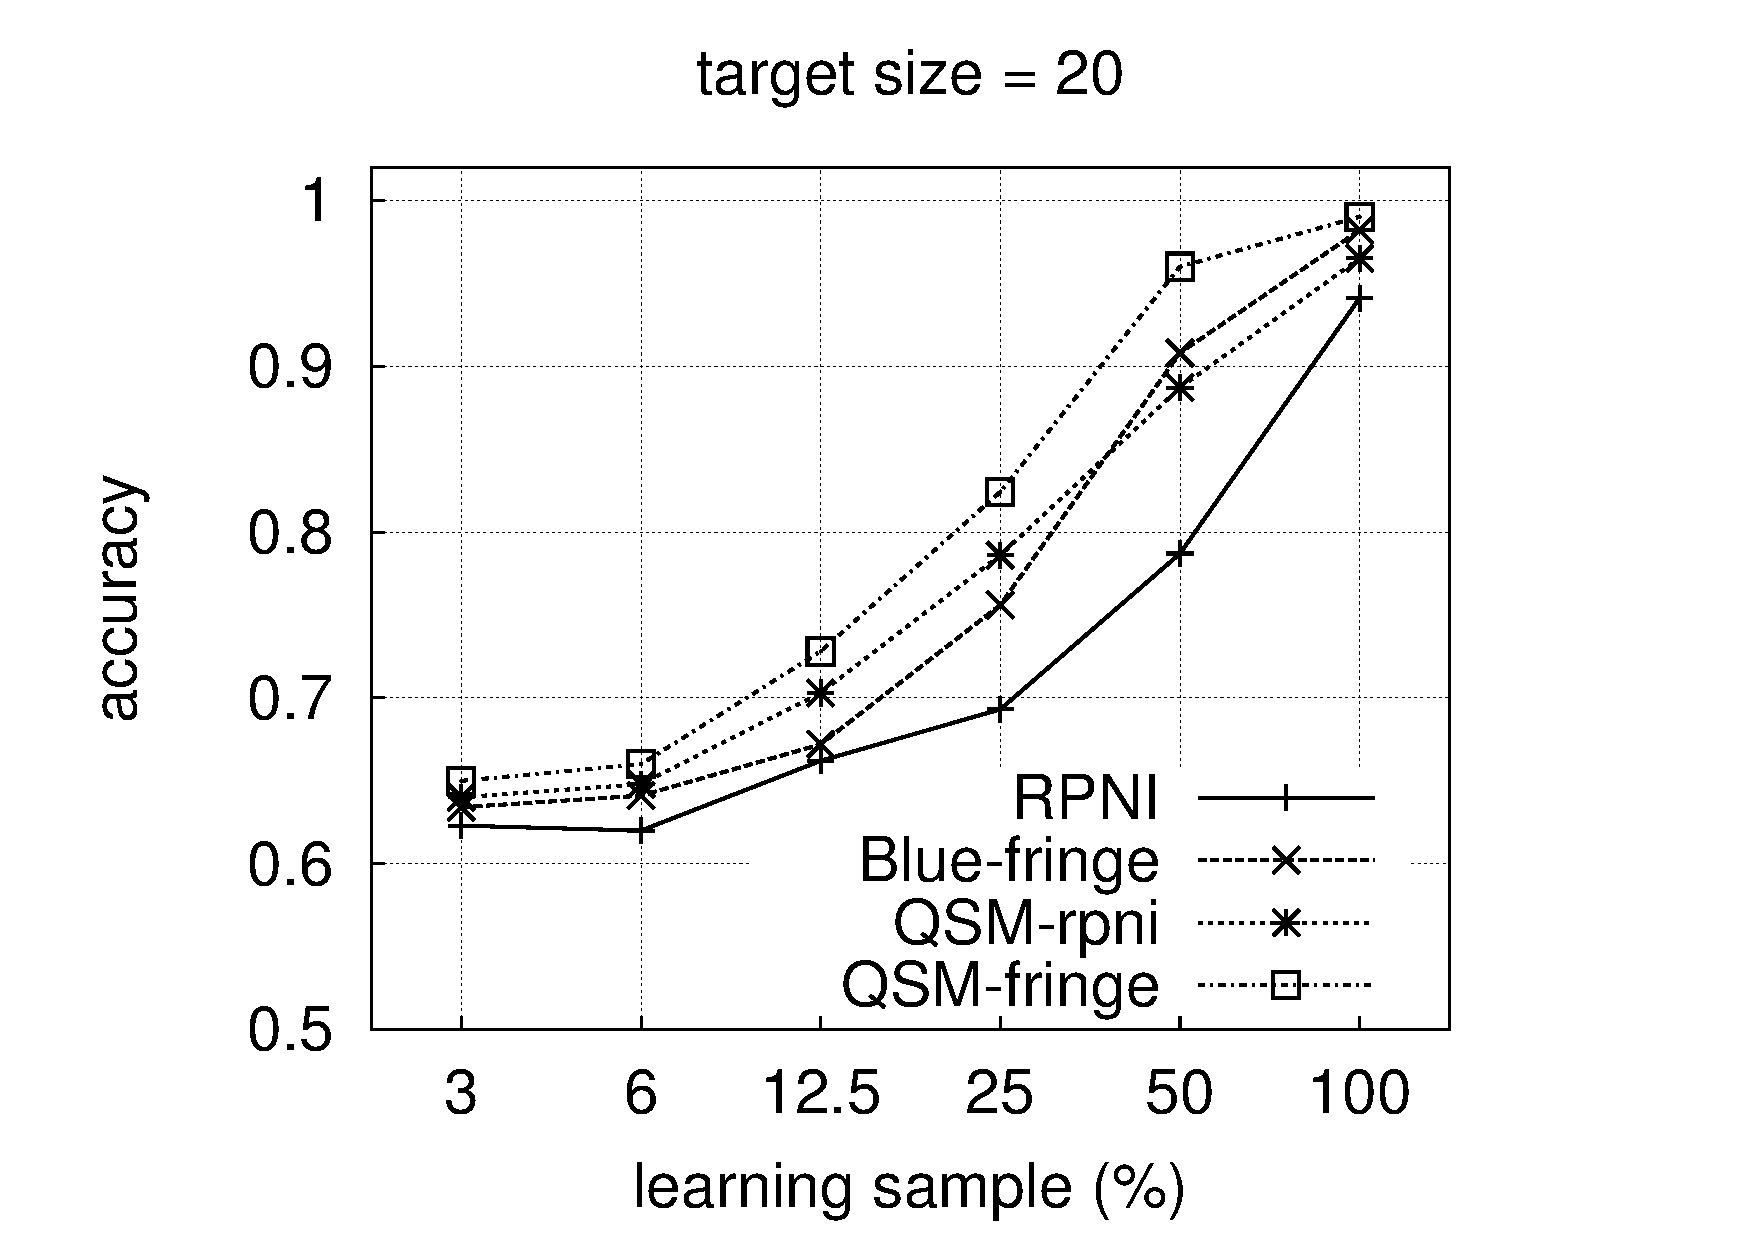
\includegraphics[trim=0mm  21mm 35mm 0mm, clip, page=1]{src/5-evaluation/images/accuracy}
  \includegraphics[trim=25mm 21mm 35mm 0mm, clip, page=2]{src/5-evaluation/images/accuracy}
  \includegraphics[trim=25mm 21mm 35mm 0mm, clip, page=3]{src/5-evaluation/images/accuracy}
}
\end{figure}

\vspace{-0cm}
{\noindent\small\sc Time}
\vspace{-0cm}

\begin{figure}[H]\centering
\scalebox{.17}{
  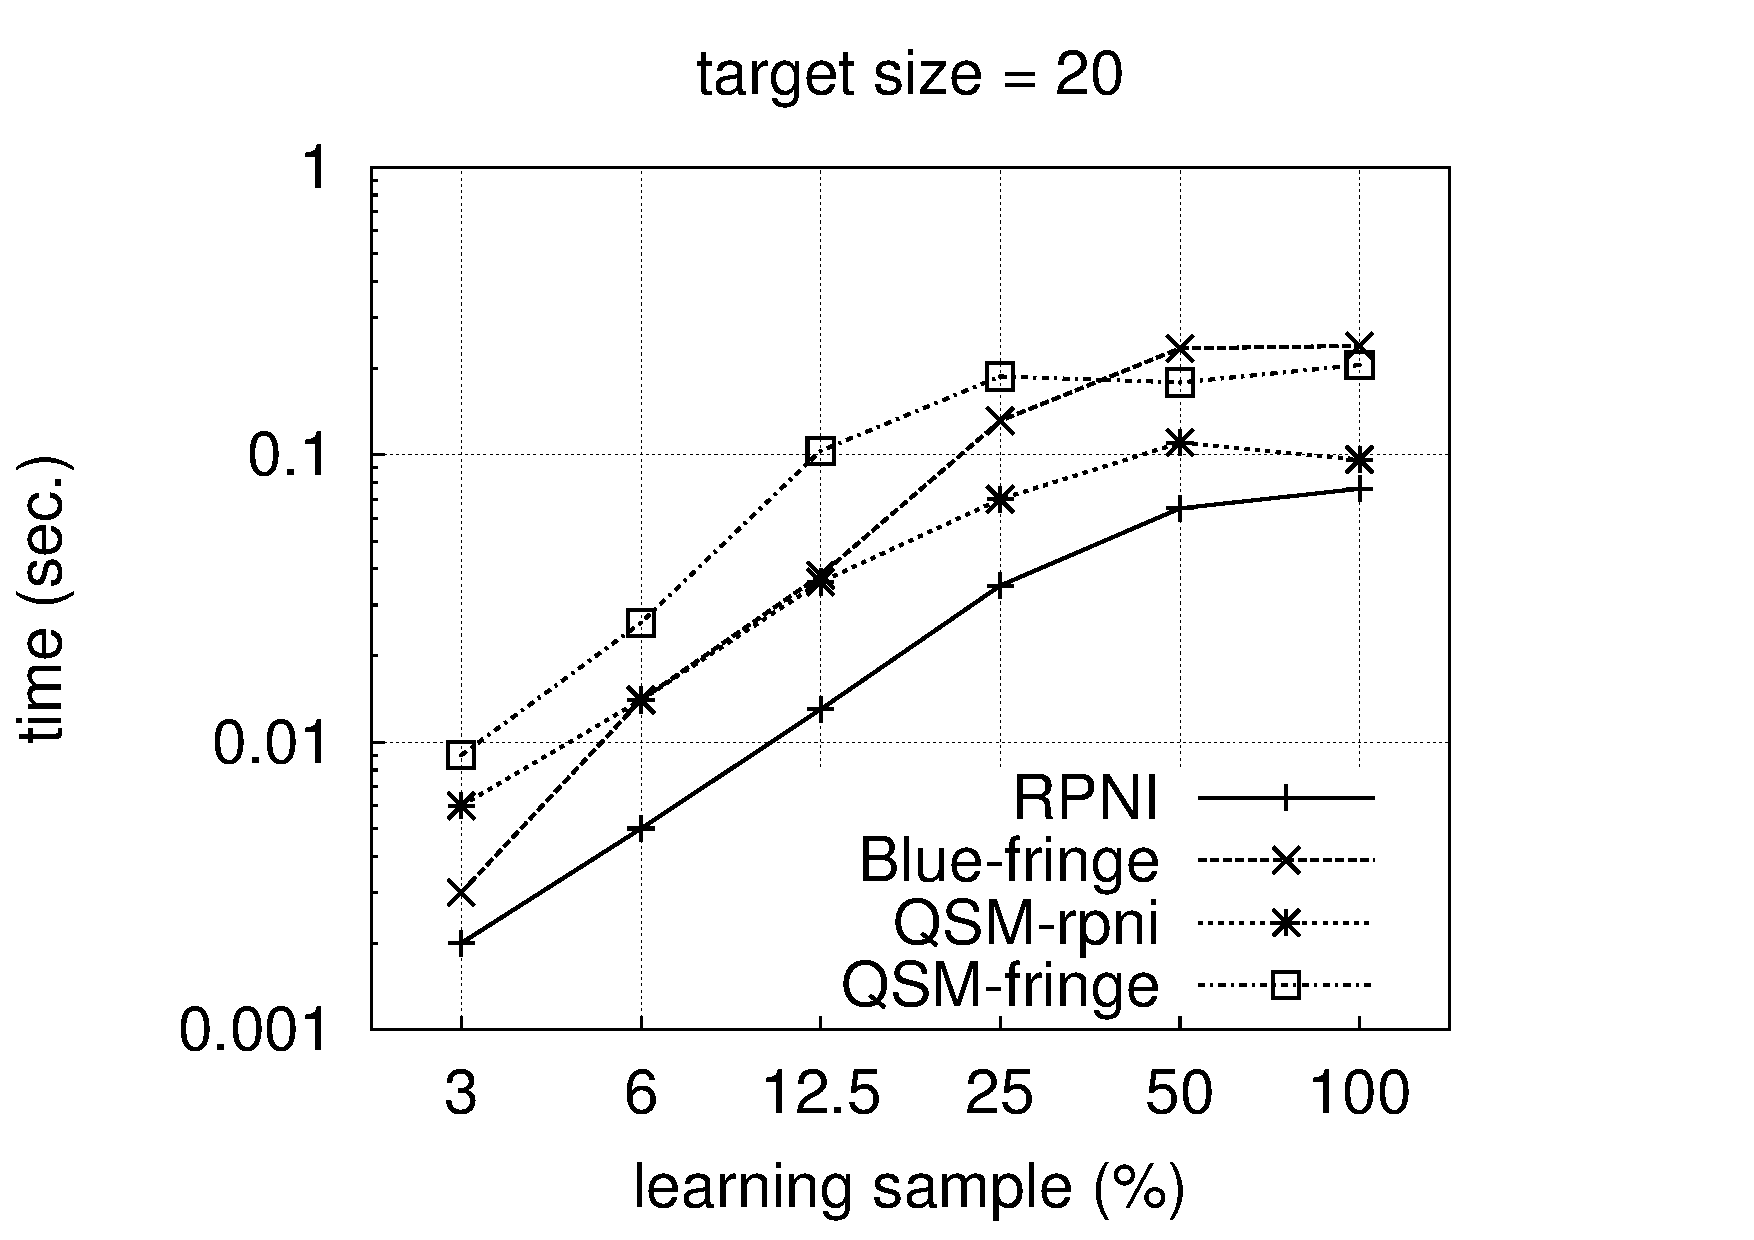
\includegraphics[trim=0mm  21mm 35mm 0mm, clip, page=1]{src/5-evaluation/images/time}
  \includegraphics[trim=25mm 21mm 35mm 0mm, clip, page=2]{src/5-evaluation/images/time}
  \includegraphics[trim=25mm 21mm 35mm 0mm, clip, page=3]{src/5-evaluation/images/time}
}
\end{figure}

\vspace{-0cm}
{\noindent\small\sc Number of queries}
\vspace{-0cm}

\begin{figure}[H]\centering
\scalebox{.17}{
  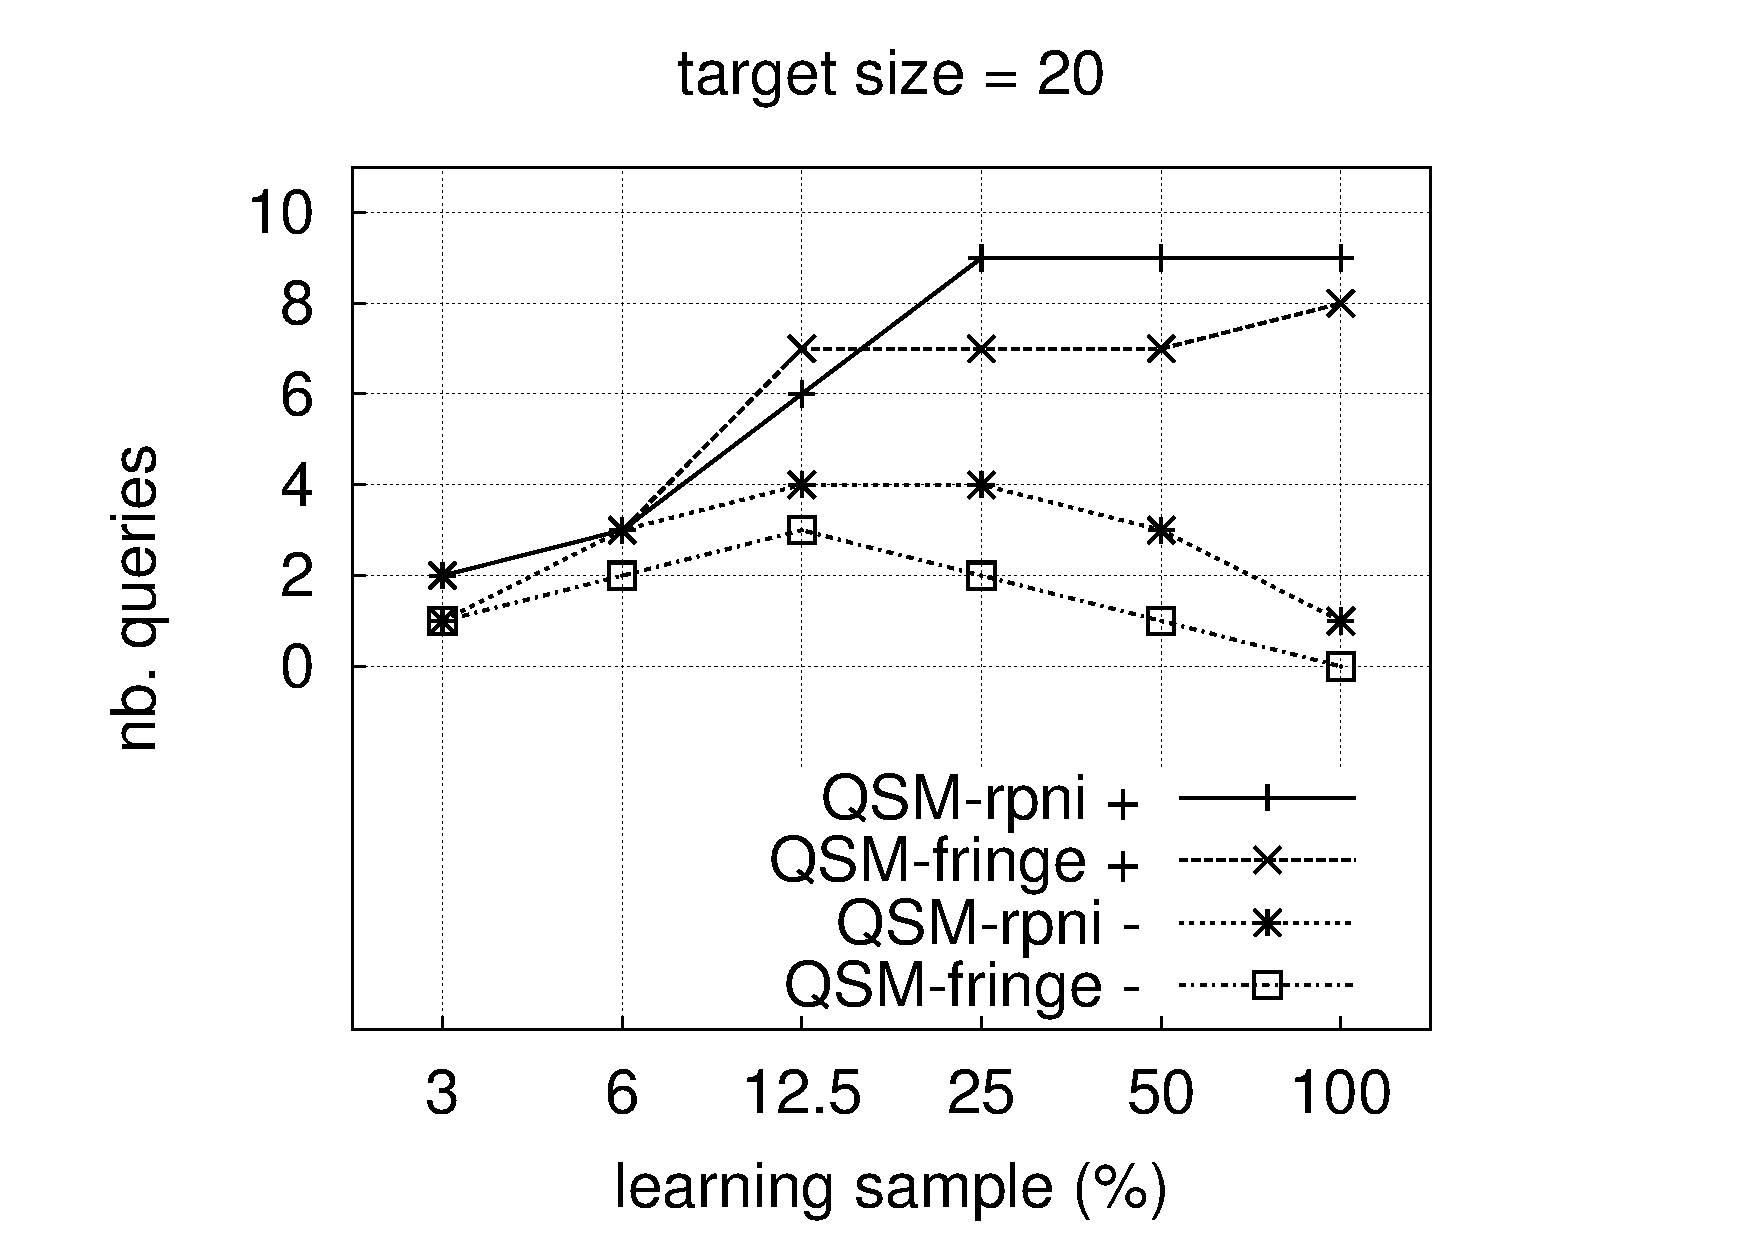
\includegraphics[trim=0mm  21mm 35mm 0mm, clip, page=1]{src/5-evaluation/images/queries}
  \includegraphics[trim=25mm 21mm 35mm 0mm, clip, page=2]{src/5-evaluation/images/queries}
  \includegraphics[trim=25mm 21mm 35mm 0mm, clip, page=3]{src/5-evaluation/images/queries}
}
\end{figure}


%%%%%%%%%%%%%%%%%%%%%%%%%%%%%%%%%%%%%%%%%%%%%%%%%%%%%%%%%%%%%%%%%%%%%%%%%%%%%%%%
\vfill
\subsection{Accuracy}

\vspace{-0cm}
{\noindent\small\sc Evidence-driven Merging}
\vspace{-0cm}

\begin{figure}[H]\centering
\scalebox{.17}{
  \includegraphics[trim=0mm  21mm 35mm 20mm, clip, page=5]{src/5-evaluation/images/accuracy}
  \includegraphics[trim=25mm 21mm 35mm 20mm, clip, page=6]{src/5-evaluation/images/accuracy}
  \includegraphics[trim=25mm 21mm 35mm 20mm, clip, page=7]{src/5-evaluation/images/accuracy}
}
\scalebox{.17}{
  \includegraphics[trim=0mm  21mm 35mm 20mm, clip, page=17]{src/5-evaluation/images/accuracy}
  \includegraphics[trim=25mm 21mm 35mm 20mm, clip, page=18]{src/5-evaluation/images/accuracy}
  \includegraphics[trim=25mm 21mm 35mm 20mm, clip, page=19]{src/5-evaluation/images/accuracy}
}
\end{figure}

\vspace{-0cm}
{\noindent\small\sc Membership queries}
\vspace{-0cm}

\begin{figure}[H]\centering
\scalebox{.17}{
  \includegraphics[trim=0mm  21mm 35mm 20mm, clip, page=9]{src/5-evaluation/images/accuracy}
  \includegraphics[trim=25mm 21mm 35mm 20mm, clip, page=10]{src/5-evaluation/images/accuracy}
  \includegraphics[trim=25mm 21mm 35mm 20mm, clip, page=11]{src/5-evaluation/images/accuracy}
}
\scalebox{.17}{
  \includegraphics[trim=0mm  21mm 35mm 20mm, clip, page=13]{src/5-evaluation/images/accuracy}
  \includegraphics[trim=25mm 21mm 35mm 20mm, clip, page=14]{src/5-evaluation/images/accuracy}
  \includegraphics[trim=25mm 21mm 35mm 20mm, clip, page=15]{src/5-evaluation/images/accuracy}
}
\end{figure}

\vspace{-0cm}
{\noindent\small\sc Control information}
\vspace{-0cm}

\begin{figure}[H]\centering
\scalebox{.17}{
  \includegraphics[trim=0mm   0mm 35mm 20mm, clip, page=9]{src/5-evaluation/images/accuracy}
  \includegraphics[trim=25mm  0mm 35mm 20mm, clip, page=10]{src/5-evaluation/images/accuracy}
  \includegraphics[trim=25mm  0mm 35mm 20mm, clip, page=11]{src/5-evaluation/images/accuracy}
}
\end{figure}


%%%%%%%%%%%%%%%%%%%%%%%%%%%%%%%%%%%%%%%%%%%%%%%%%%%%%%%%%%%%%%%%%%%%%%%%%%%%%%%%

\vfill
\subsection{Time}

\vspace{-0cm}
{\noindent\small\sc Evidence-driven Merging}
\vspace{-0cm}

\begin{figure}[H]\centering
\scalebox{.17}{
  \includegraphics[trim=0mm  21mm 35mm 20mm, clip, page=5]{src/5-evaluation/images/time}
  \includegraphics[trim=25mm 21mm 35mm 20mm, clip, page=6]{src/5-evaluation/images/time}
  \includegraphics[trim=25mm 21mm 35mm 20mm, clip, page=7]{src/5-evaluation/images/time}
}
\scalebox{.17}{
  \includegraphics[trim=0mm  21mm 35mm 20mm, clip, page=17]{src/5-evaluation/images/time}
  \includegraphics[trim=25mm 21mm 35mm 20mm, clip, page=18]{src/5-evaluation/images/time}
  \includegraphics[trim=25mm 21mm 35mm 20mm, clip, page=19]{src/5-evaluation/images/time}
}
\end{figure}

\vspace{-0cm}
{\noindent\small\sc Membership queries}
\vspace{-0cm}

\begin{figure}[H]\centering
\scalebox{.17}{
  \includegraphics[trim=0mm  21mm 35mm 20mm, clip, page=9]{src/5-evaluation/images/time}
  \includegraphics[trim=25mm 21mm 35mm 20mm, clip, page=10]{src/5-evaluation/images/time}
  \includegraphics[trim=25mm 21mm 35mm 20mm, clip, page=11]{src/5-evaluation/images/time}
}
\scalebox{.17}{
  \includegraphics[trim=0mm  21mm 35mm 20mm, clip, page=13]{src/5-evaluation/images/time}
  \includegraphics[trim=25mm 21mm 35mm 20mm, clip, page=14]{src/5-evaluation/images/time}
  \includegraphics[trim=25mm 21mm 35mm 20mm, clip, page=15]{src/5-evaluation/images/time}
}
\end{figure}

\vspace{-0cm}
{\noindent\small\sc Control information}
\vspace{-0cm}

\begin{figure}[H]\centering
\scalebox{.17}{
  \includegraphics[trim=0mm   0mm 35mm 20mm, clip, page=9]{src/5-evaluation/images/time}
  \includegraphics[trim=25mm  0mm 35mm 20mm, clip, page=10]{src/5-evaluation/images/time}
  \includegraphics[trim=25mm  0mm 35mm 20mm, clip, page=11]{src/5-evaluation/images/time}
}
\end{figure}


%%%%%%%%%%%%%%%%%%%%%%%%%%%%%%%%%%%%%%%%%%%%%%%%%%%%%%%%%%%%%%%%%%%%%%%%%%%%%%%%
\vfill
\subsection{Number of queries}

\vspace{-0cm}
{\noindent\small\sc Evidence-driven merging}
\vspace{-0cm}

\begin{figure}[H]\centering
\scalebox{.17}{
  \includegraphics[trim=0mm  21mm 35mm 20mm, clip, page=5]{src/5-evaluation/images/queries}
  \includegraphics[trim=25mm 21mm 35mm 20mm, clip, page=6]{src/5-evaluation/images/queries}
  \includegraphics[trim=25mm 21mm 35mm 20mm, clip, page=7]{src/5-evaluation/images/queries}
}
\scalebox{.17}{
  \includegraphics[trim=0mm  21mm 35mm 20mm, clip, page=9]{src/5-evaluation/images/queries}
  \includegraphics[trim=25mm 21mm 35mm 20mm, clip, page=10]{src/5-evaluation/images/queries}
  \includegraphics[trim=25mm 21mm 35mm 20mm, clip, page=11]{src/5-evaluation/images/queries}
}
\end{figure}

